\hyphenation{wnio-sko-wa-nie}
\chapter{Problematyka automatycznego planowania}
 \section{Opis dziedziny}
 \label{sec:opis}
Automatyczne planowanie to poddziedzina sztucznej inteligencji, która dotyczy wykonywania sekwencji akcji, realizacji strategii lub generowania planów, prowadzących do określonego wyniku \cite{planning}.

Każdy problem automatycznego planowania zawiera stan początkowy oraz stan końcowy. W stanie początkowym określone są wszystkie wartości zmiennych (stany poszczególnych obiektów) jakie aktualnie zawarte są w problemie, a które mają zostać zmienione podczas wykonania planu. W stanie końcowym sformułowane są wartości zmiennych, których osiągniecie jest głównym zadaniem planu. Ponadto problemy automatycznego planowania zawierają zdefiniowane operatory, umożliwiające zmianę stanu. Tylko przez podejmowanie akcji plan może zostać wykonany. Wyjątkiem jest sytuacja, w której stan końcowy jest równy stanu początkowemu.

Plany, otrzymywane w wyniku rozwiązywania problemów, można otrzymać dzięki zastosowaniu różnego rodzaju schematów działania. Spośród klasycznych algorytmów, wymienić można między innymi całkowity przegląd stanów, wnioskowanie w tył czy wnioskowanie w przód. Mimo, iż całkowity przegląd stanów zapewni rozwiązanie najlepsze, jest to rzadko stosowane rozwiązanie. Liczba stanów możliwych do osiągnięcia rośnie wykładniczo, co powoduje, że proces planowania nawet niezbyt skomplikowanych problemów, może zająć czas niewspółmierny do osiągniętych rezultatów. W takim wypadku stosuje się algorytmy mogące zwrócić plany, których wykonanie zajmie więcej czasu, jednak szybkość ich uzyskania znacznie wzrasta \cite{fdalgorytm}.

Pomimo osiągania satysfakcjonujących wyników przez algorytmy klasyczne, wykorzystywane jest również kilka bardziej złożonych rozwiązań. Jednym z nich jest przekształcenie danego problemu automatycznego planowania w instancję problemu spełnialności formuły logicznej (wynikającej z pierwotnego problemu)\JP{rachunku zdań czy predykatów? trzeba to doprecyzować, bo to znacząco zmienia klasę złożoności}, a następnie  rozwiązanie go najlepszą znaną metodą. Kolejnym wyjściem są algorytmy probabilistyczne. Polegają one na polepszaniu wyników podczas kolejnych iteracji. Algorytmy te wykonują akcje z określonym prawdopodobieństwem, przez co, może się okazać, że optymalny plan zostanie uzyskany później niż w przypadku pełnego przeglądu stanów, lub nawet nie zostanie uzyskany nigdy. Na ogół jednak, algorytmy probabilistyczne dostarczają wyniki porównywalne z algorytmami klasycznymi, w nie gorszym czasie.

Bardzo często, w celu zaprezentowania czym jest automatyczne planowanie, stosuje się układ złożony z klocków, umiejscowionych w określonej pozycji. Zadaniem algorytmów planowania jest takie ułożenie akcji, aby stan końcowy położenia klocków zgadzał się z wcześniej ustalonymi założeniami.\JP{Tu możnaby odwołać się do pracy, w której to pojawiło się po raz pierwszy:  Gupta, Naresh, and Dana S. Nau. "On the complexity of blocks-world planning." Artificial Intelligence 56.2 (1992): 223-254.}

Przykładowo, istnieją 3 klocki, nazwane odpowiednio $x$, $y$, $z$. Każdy z nich może być podniesiony lub umiejscowionym na jednym z dwóch dostępnych miejsc ($M1$, $M2$) lub na innym klocku, pod warunkami, że ten nie jest akurat podniesiony i nic się na nim nie znajduje. Dla danego problemu zdefiniowane zostały akcje \emph{podnieś}, która podnosi dany klocek, oraz \emph{połóż}, dzięki której można umiejscowić klocek na wolnym miejscu lub innym klocku. Stan początkowy zdefiniowany jest następująco: klocek $z$ położony jest na pierwszym miejscu, klocek $y$ położony jest na klocku $z$, a klocek $x$ na klocku $y$. Stan końcowy wygląda tak, że klocek $x$ znajduje się na miejscu drugim, na nim umiejscowiony jest klocek $y$, a z kolei na nim klocek $z$. Inaczej można przedstawić to w języku predykatów:
\\\\
Stan początkowy:
\\\\
\textit{P=\{wolny(x),na(x,y),na(y,z),na(z,M1)\}}
\\\\
Stan końcowy:
\\\\
\textit{K=\{wolny(z),na(z,y),na(y,x),na(x,M2)\}}

Na rysunku \ref{fig:automatyczne-planowanie} przedstawiono graficzne odwzorowanie stanu początkowego i końcowego.
\begin{figure}[h!]
    \centering
    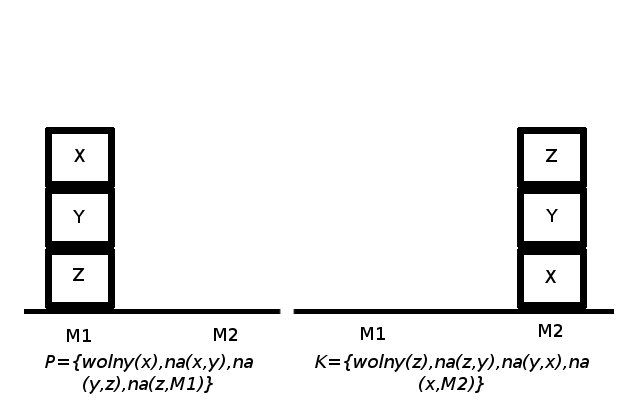
\includegraphics[width=0.5\textwidth]{img/rys2,1}
    \caption{Graficzna reprezentacja stanu początkowego i końcowego}
    \label{fig:automatyczne-planowanie}
\end{figure}


\section{Język PDDL}
\label{sec:jezykpddl}
Na potrzeby automatycznego planowania, stworzone zostało kilka formalnych języków, dedykowanych specjalnie dla tej dziedziny. Najpopularniejsze z nich to STRIPS (ang. \textit{\textbf{St}anford \textbf{R}esearch \textbf{I}nstitute \textbf{P}roblem \textbf{S}olver}) \cite{strips}, ADL (ang. \textit{Action description language}) \cite{adl} oraz PDDL (ang. \textit{Planning Domain Definition Language}) \cite{pddl}. PDDL, który powstał najpóźniej, jest wzorowany na dwóch pozostałych językach. Został stworzony przez Drew McDermott'a w roku 1998 z przeznaczeniem na Międzynarodowy Konkurs Planistyczny (ang. \textit{International Planning Competition}), który bez odpowiedniego narzędzia nie mógłby się odbyć.

Od pojawienia się pierwszej wersji języka w roku 1998, jest on systematycznie rozwijany. Kolejne wersje 2.1, 2.2, 3.0, oraz najnowsza 3.1 zostały użyte na międzynarodowych konkursach w latach 2002, 2004, 2006, 2008. Oprócz standardowych wersji języka, rozwijane są inne, niezależne warianty. Pośród nich znajdują się między innymi PDDL+, w~którym zawarto procesy i zdarzenia \cite{pddlplus}, \emph{Web-PDDL} umożliwiający wyrażenie przestrzeni nazw za pomocą URI (ang. \textit{Uniform Resource Identifier}) \cite{webpddl}, czy NDDL (ang. \textit{New Domain Definition Language}), różniący się używaniem zmiennych oraz interwałów zamiast akcji \cite{npdl}.

Problemy automatycznego planowania, przedstawione w języku PDDL, są zapisane w~dwóch plikach, dziedziny oraz problemu. Poniżej przedstawiono skrócony opis obydwu plików. Składa się on z przedstawienia elementu, krótkiego opisu oraz przykładu.
\\\\\\
Plik dziedziny zawiera:
  \begin{description}
\item[Dziedzina] Definicja dziedziny: \texttt{(define (domain samoloty))}
\item[Rozszerzenie] Dziedzina zawierająca dany wpis dziedziczy wymagania, typy, stałe, akcje, aksjomaty z innej dziedziny: \texttt{(:extends pojazdy) }
\item[Wymagania] Fragmenty języka PDDL wykorzystywane przez opis dziedziny: \texttt{(:requirements :strips :typing)}
\item[Typy] Typy znajdujące się w problemie: \texttt{(:types okno drzwi)}
\item[Stałe] Zdefiniowane stałe: \texttt{(:constants pierwsza druga - opona)}
\item[Zmienne dziedzinowe] Zmienne dla dziedzin, które mają zadeklarowe wymaganie \texttt{:expression-evaluation}: \texttt{(:domain-variables zmienna - int)}
\item[Predykaty] Lista predykatów zawartych w dziedzinie (znak \texttt{?} poprzedzający \texttt{x} oznacza, że \texttt{x} jest zmienną):  \texttt{  (:predicates 
   (połaczone-z-lad ?p1 - miejsce ?p2 - miejsce) 
   (połaczone-z-droga ?p1 - miejsce ?p2 - miejsce) 
   (połaczone-z-morze ?p1 - miejsce ?p2 - miejsce) 
   (las ?p - miejsce) 
   (gora ?p - miejsce) )}
\item[Pola wieczne] Lista literałów, które są prawdziwe w każdej chwili: \texttt{(:timeless literał (nazwa))}
\item[Ograniczenia bezpieczeństwa] Ograniczenia, które muszą pozostać spełnione w każdym punkcie tworzonego planu: \texttt{(:safety (:goal (na-lotnisku samolot))}
\item[Operatory] Lista operatorów, których podejmowanie ma zapewnić osiągnięcie celu. Każdy operator zawiera warunki wykonania, parametry oraz efekt, jaki powinien przynieść: \texttt{(:action laduj :parameters (?s - samolot ?l - lotnisko ?p - powietrze) :precondition (jest-na ?s ?p) :effect (jest-na ?s ?l)) }\\
\end{description}


Plik problemu zawiera:
\begin{description}
\item[Dziedzina] Wskazanie, do której dziedziny odnosi się definiowany problem: \texttt{(:domain loty)}
\item[Wymagania] Fragmenty języka PDDL wykorzystywane przez opis dziedziny: \texttt{(:requirements :strips :typing)}
\item[Sytuacja] Nazwa sytuacji początkowej: \texttt{(:situation początek)}
\item[Obiekty] Lista obiektów występujących w problemie: \texttt{(:objects drzewo liść)}
\item[Stan początkowy] Opis stanu początkowego problemu w formie listy spełnionych literałów: \texttt{(:init (jest A) (w B hangar))}
\item[Cel] Oczekiwany stan końcowy problemu w formie formuły logicznej, która musi być spełniona: \texttt{(:goal (and (jest A) (w C hangar) (w B lotnisko))}
\item[Długość rozwiązania] Pole stwierdzające, iż istnieje rozwiązanie o podanej długości: \texttt{(:length (:serial 5))}
\end{description}
\begin{Code}
\begin{lstlisting}[language=LISP,frame=single,label=ana_code, caption=Zawartość przykładowego pliku dziedziny]
(define (domain loty)
(:extends pojazdy)
(:requirements :strips :typing )
(:predicates
	(lotnisko ?m - miejsce)
	(powietrze ?m - miejsce)
	(samolot	?p - pojazd)
	(jest-na ?p - pojazd ?m - miejsce)
)
(:action laduj
	:parameters (?s - samolot ?m - miejsce)
   	:precondition (is-at ?s ?m) 
	:effect (jest-na ?s ?m) 
)
)
\end{lstlisting}
\end{Code}

\begin{Code}
\begin{lstlisting}[language=LISP,frame=single,label=ana_code, caption=Zawartość przykładowego pliku problemu]
(define (problem lotniska-start)
	(:domain lotniska)
	(:situation ladowanie)
	(:init (at B hangar) (at A lotnisko))
	(:goal (and(at A hangar) (at B lotnisko))))
\end{lstlisting}
\end{Code}

Aby stworzyć w pełni funkcjonalną wtyczkę, należało przygotować gramatykę formalną, Jest to zbór wszystkich symboli leksykalnych, zwanych \emph{symbolami terminalnymi, symboli nieterminalnych} oraz reguł, określających sposób wyprowadzania słów, należących do języka PDDL. Bez gramatyki niemożliwe byłoby wykonanie większości funkcji, które powinny być zapewnione przez GUI4PDDL. \JP{Bardzo to enigmatycznie brzmi. Może niech pojawi się tu jakiś odnośnik do rozdziału, gdzie to jest szczegółowo opisane.}

\section{Oprogramowanie}
\label{sec:oprogramowanie}
Język PDDL jest wspierany przez wiele narzędzi, służących do przeprowadzania procesu planowania. Jednym z takich narządzi jest \textit{Fast Downward}\footnote{\url{http://www.fast-downward.org/}}\JP{Malte Helmert. The Fast Downward Planning System. Journal of Artificial Intelligence Research 26, pp. 191-246. 2006.}, który pozwala na zaplanowanie problemu zapisanego w~jęzeku PDDL w wersji 2.2. Dodatkowo wspiera wymaganie \textit{:action-costs}, wprowadzone w wersji 3.1. Aplikacja wymaga od użytkownika posiadania dostępu do wiersza poleceń oraz prostego edytora tekstu. Do ułożenia planu \textit{Fast Downward} używa heurystyki opartej na kilku algorytmach, między innymi \textit{Best-First Search} \cite{fdalgorytm}. Na podobnej zasadzie działania oparte są aplikacje \textit{Fast Forward}\footnote{\url{http://fai.cs.uni-saarland.de/hoffmann/ff.html}}\JP{B. Nebel, The FF Planning System: Fast Plan Generation Through Heuristic Search, in: Journal of Artificial Intelligence Research, Volume 14, 2001, Pages 253 - 302.} oraz \textit{LPG}\footnote{\url{http://zeus.ing.unibs.it/lpg/}}\JP{Alfonso Gerevini and Ivan Serina, "LPG: a Planner based on Local Search for Planning Graphs", in Proceedings of the Sixth International Conference on Artificial Intelligence Planning and Scheduling (AIPS'02), AAAI Press, Toulouse, France, 2002.}.

Kolejny planer nosi nazwę \textit{SatPlan}\footnote{\url{http://www.cs.rochester.edu/users/faculty/kautz/satplan/index.htm}}\JP{SatPlan: Planning as Satisfiability
Henry Kautz, Bart Selman, and Joerg Hoffmann. Abstracts of the 5th International Planning Competition, 2006.}. Algorytm wykorzystywany przez ten program spełnia założenia metody automatycznego planowania o takiej samej nazwie: konwertuje daną instancję problemu planowania na instancję problemu spełnialności formuły logicznej, a następnie rozwiązuje, wykorzystując odpowiednie schematy działań \cite{satplan}. Algorytm zawarty w \textit{SatPlan'ie} ma następujący przebieg: 

  \begin{enumerate}
\item Na podstawie problemu automatycznego planowania tworzy się graf o pewnej długości \textit{k}.
\item Ograniczenia wynikające z grafu zamieniane są na zbiór klauzul.
\item Przy użyciu odpowiedniego algorytmu, pozwalającego rozstrzygnąć problem spełnialności danego zbioru klauzul, znajduje się odpowiednie rozwiązanie.
\item W przypadku gdy nie można było znaleźć wyniku, zwiększona zostaje wartość \textit{k}.
\item Jeżeli rozwiązanie zostało znalezione, przekształca się wynik działania algorytmu do wyniku pierwotnego problemu planowania.
\item Na końcu usuwane są niektóre z niepotrzebnych akcji.
\end{enumerate}


Kolejną aplikacją umożliwiającą rozwiązywanie problemów automatycznego planowania jest Gavs+ (\textit{Game Arena Visualization and Synthesis, Plus!})\footnote{\url{http://www6.in.tum.de/~chengch/gavs/}}, który skupia się na kwestiach związanych z grami. Program ten posiada bibliotekę (\textit{PDDL4J}) umożliwiającą wykonywanie problemów zapisanych w PDDL. Dzięki wbudowanemu interfejsowi Gavs+ umożliwia graficzne prześledzenie wynikowego planu.

Wszystkie opisane tu narzędzia opublikowane zostały na licencji otwartego oprogramowania.

%algorytmy używane przez planery
%satplan
%gavs +
